\documentclass[xcolor=dvipsnames]{beamer}
\usepackage[T1]{fontenc}
\usepackage[utf8]{inputenc}
\usepackage[english,slovak]{babel}

\usepackage{amsmath}
\usepackage{amsthm}
\usetheme{Pittsburgh}
\useoutertheme{shadow}

\usepackage{graphicx}
\usepackage{caption}
\usepackage{subcaption}

\usepackage[]{algorithm2e}
\usepackage{listings}
 \setbeamercovered{transparent}
 \usepackage{cuted}
\usepackage[export]{adjustbox}
\usepackage{mathtools}

\usepackage{lipsum}
\usepackage{verbatim}
\usepackage{transparent}
\usepackage{framed}
\usepackage{xcolor}

\usepackage{multirow}
\usepackage{colortbl}
\usepackage{lmodern}

\usepackage{hyperref}

\usepackage{movie15}


\iftrue

\usetheme{Warsaw}

\setbeamercolor{normal text}{fg=white,bg=black!90}
\setbeamercolor{structure}{fg=white}

\setbeamercolor{alerted text}{fg=red!85!black}

\setbeamercolor{item projected}{use=item,fg=black,bg=item.fg!35}

\setbeamercolor*{palette primary}{use=structure,fg=structure.fg}
\setbeamercolor*{palette secondary}{use=structure,fg=structure.fg!95!black}
\setbeamercolor*{palette tertiary}{use=structure,fg=structure.fg!90!black}
\setbeamercolor*{palette quaternary}{use=structure,fg=structure.fg!95!black,bg=black!80}

\setbeamercolor*{framesubtitle}{fg=white}

\setbeamercolor*{block title}{parent=structure,bg=black!60}
\setbeamercolor*{block body}{fg=black,bg=black!10}
\setbeamercolor*{block title alerted}{parent=alerted text,bg=black!15}
\setbeamercolor*{block title example}{parent=example text,bg=black!15}

\fi



%-------------------------------------------------------------------------------------
\title{\color{white} \bf My research}
\author{\color{white} Michal CHOVANEC, PhD}


%\setbeamertemplate{footline}[frame number]{}
\setbeamertemplate{navigation symbols}{}


\date[EURP]{}
\begin{document}

{
    \usebackgroundtemplate
    {
        \vbox to \paperheight{\vfil\hbox to \paperwidth{\hfil

        {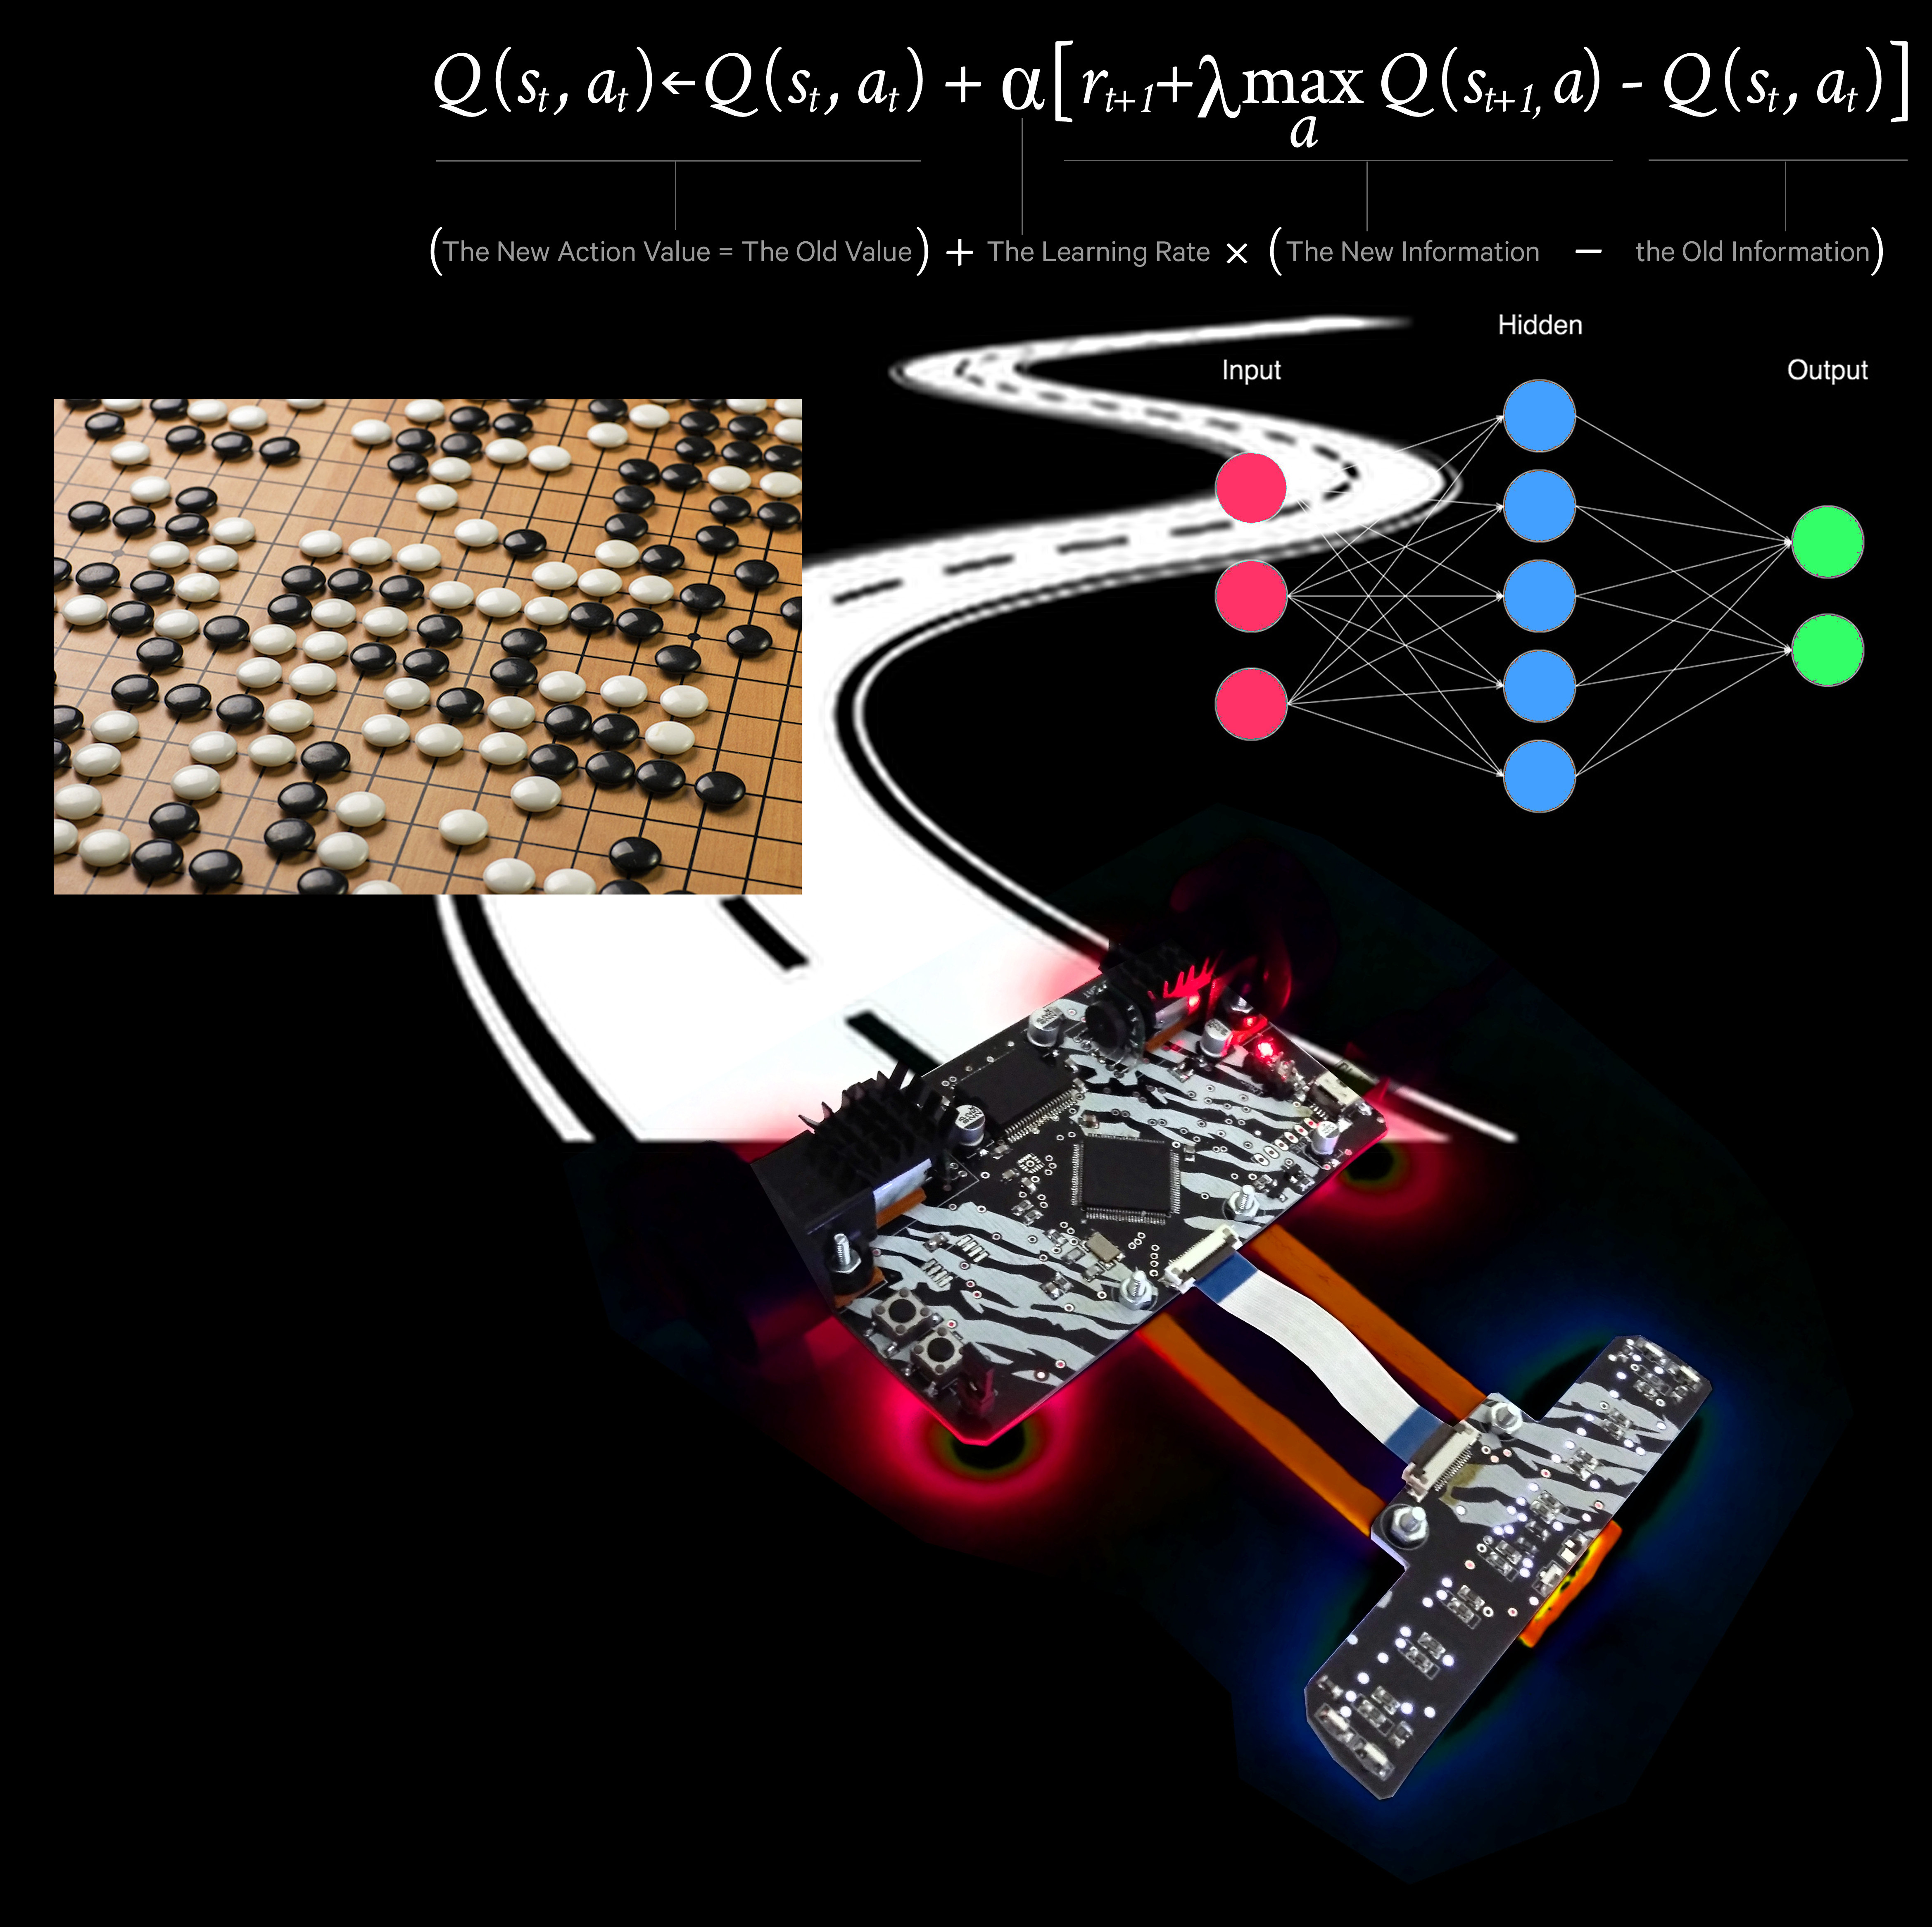
\includegraphics[width=5.05in]{../../pictures/rl_square.jpg}}

        \hfil}\vfil}
    }
    \begin{frame}

    %\titlepage


    \centering
     \colorbox{black}
     {
        \begin{minipage}{7cm}
           {\LARGE \color{white} \bf My research} \\
           {\LARGE \color{white} Michal CHOVANEC, PhD} \\
       \end{minipage}
     }


    \end{frame}
}

\begin{frame}{\bf Overview}

{\color{red} \bf my GitHub} \url{https://github.com/michalnand/}

\begin{itemize}
    \item Robotics (hobby)
    \item Red blood cells trajectory prediction
    \item Reinforcement learning
    \item education (Learning systems - methods and applications, 5II140)
\end{itemize}

{\color{red} \bf Rysy} - my own CNN framework written from scratch
{\footnotesize \url{https://github.com/michalnand/rysy}}


\begin{itemize}
    \item technologies C++17, Cuda, Python \\
        {\footnotesize - and many others : openCV, openGL, MPI, JsonCPP, cIMG, Swig, numpy, scipy, gym, ARM Cortex ...}
    \item 38 000 lines of code
    \item CNN, DenseNet
    \item deep Q networks, dueling Q networks
    \item experiments automatization (classification, regression, RL)
\end{itemize}

\end{frame}




\begin{frame}{\bf Robotics - line follower}

{\bf Curve shape classification - go faster on straight line}
\begin{columns}
    \begin{column}{0.5\textwidth}

    \begin{itemize}
      \item network architecture  \\
      {\footnotesize IN8x8x1 - C3x3x4 - P2x2 - DC3x3x4 - DC3x3x4 - FC5}
      \item {\color{red} \bf first} portable embedded DenseNet implementation
      \item running {\color{red} \bf more than 200FPS} on ARM Cortex M4 stm32f303 (72MHz)
      \item response 4..5ms
      \item network input : 8 last line sensors results (8x8 matrix)
      \item {\color{red} \bf istrobot 2016} L2 first price winner
    \end{itemize}


    \end{column}

    \begin{column}{0.5\textwidth}  %%<--- here

        \begin{figure}
          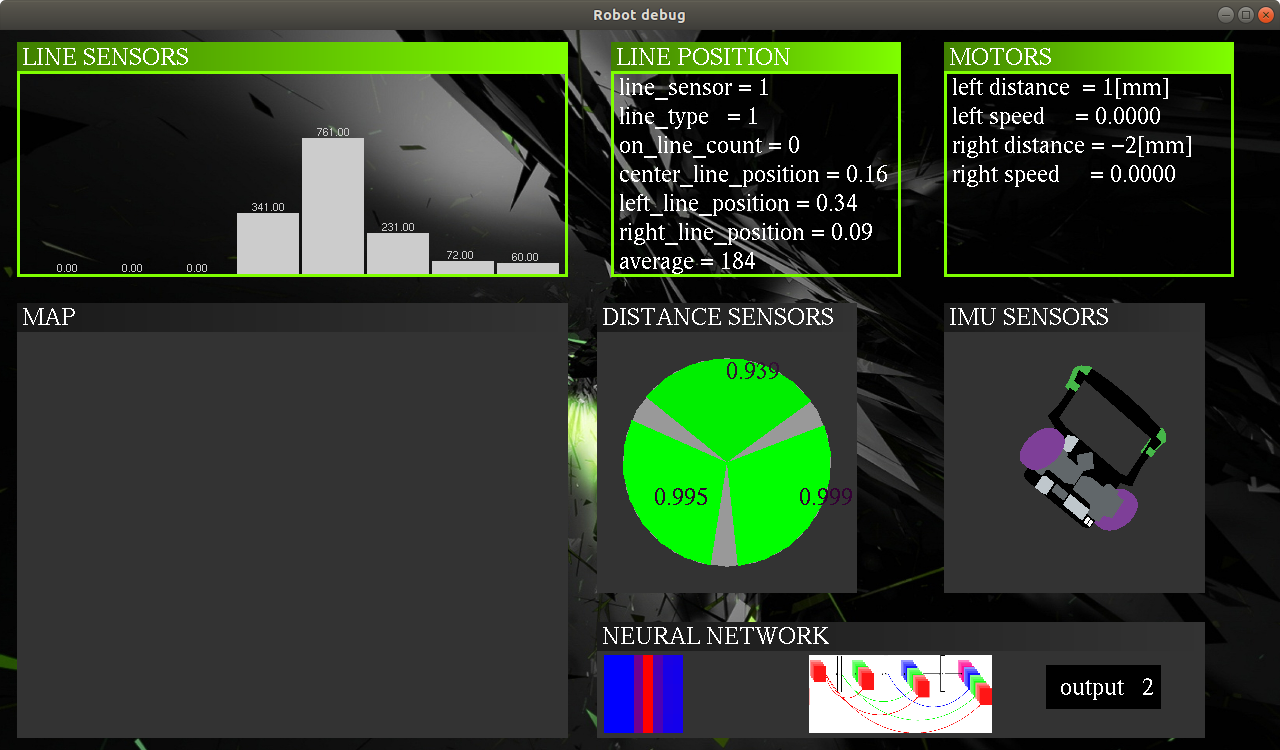
\includegraphics[scale=0.1]{../../pictures/robot_debug_app.png}
        \end{figure}

        \includemovie[
          poster,
          autoplay,
          externalviewer,
          inline=false,
          text={ 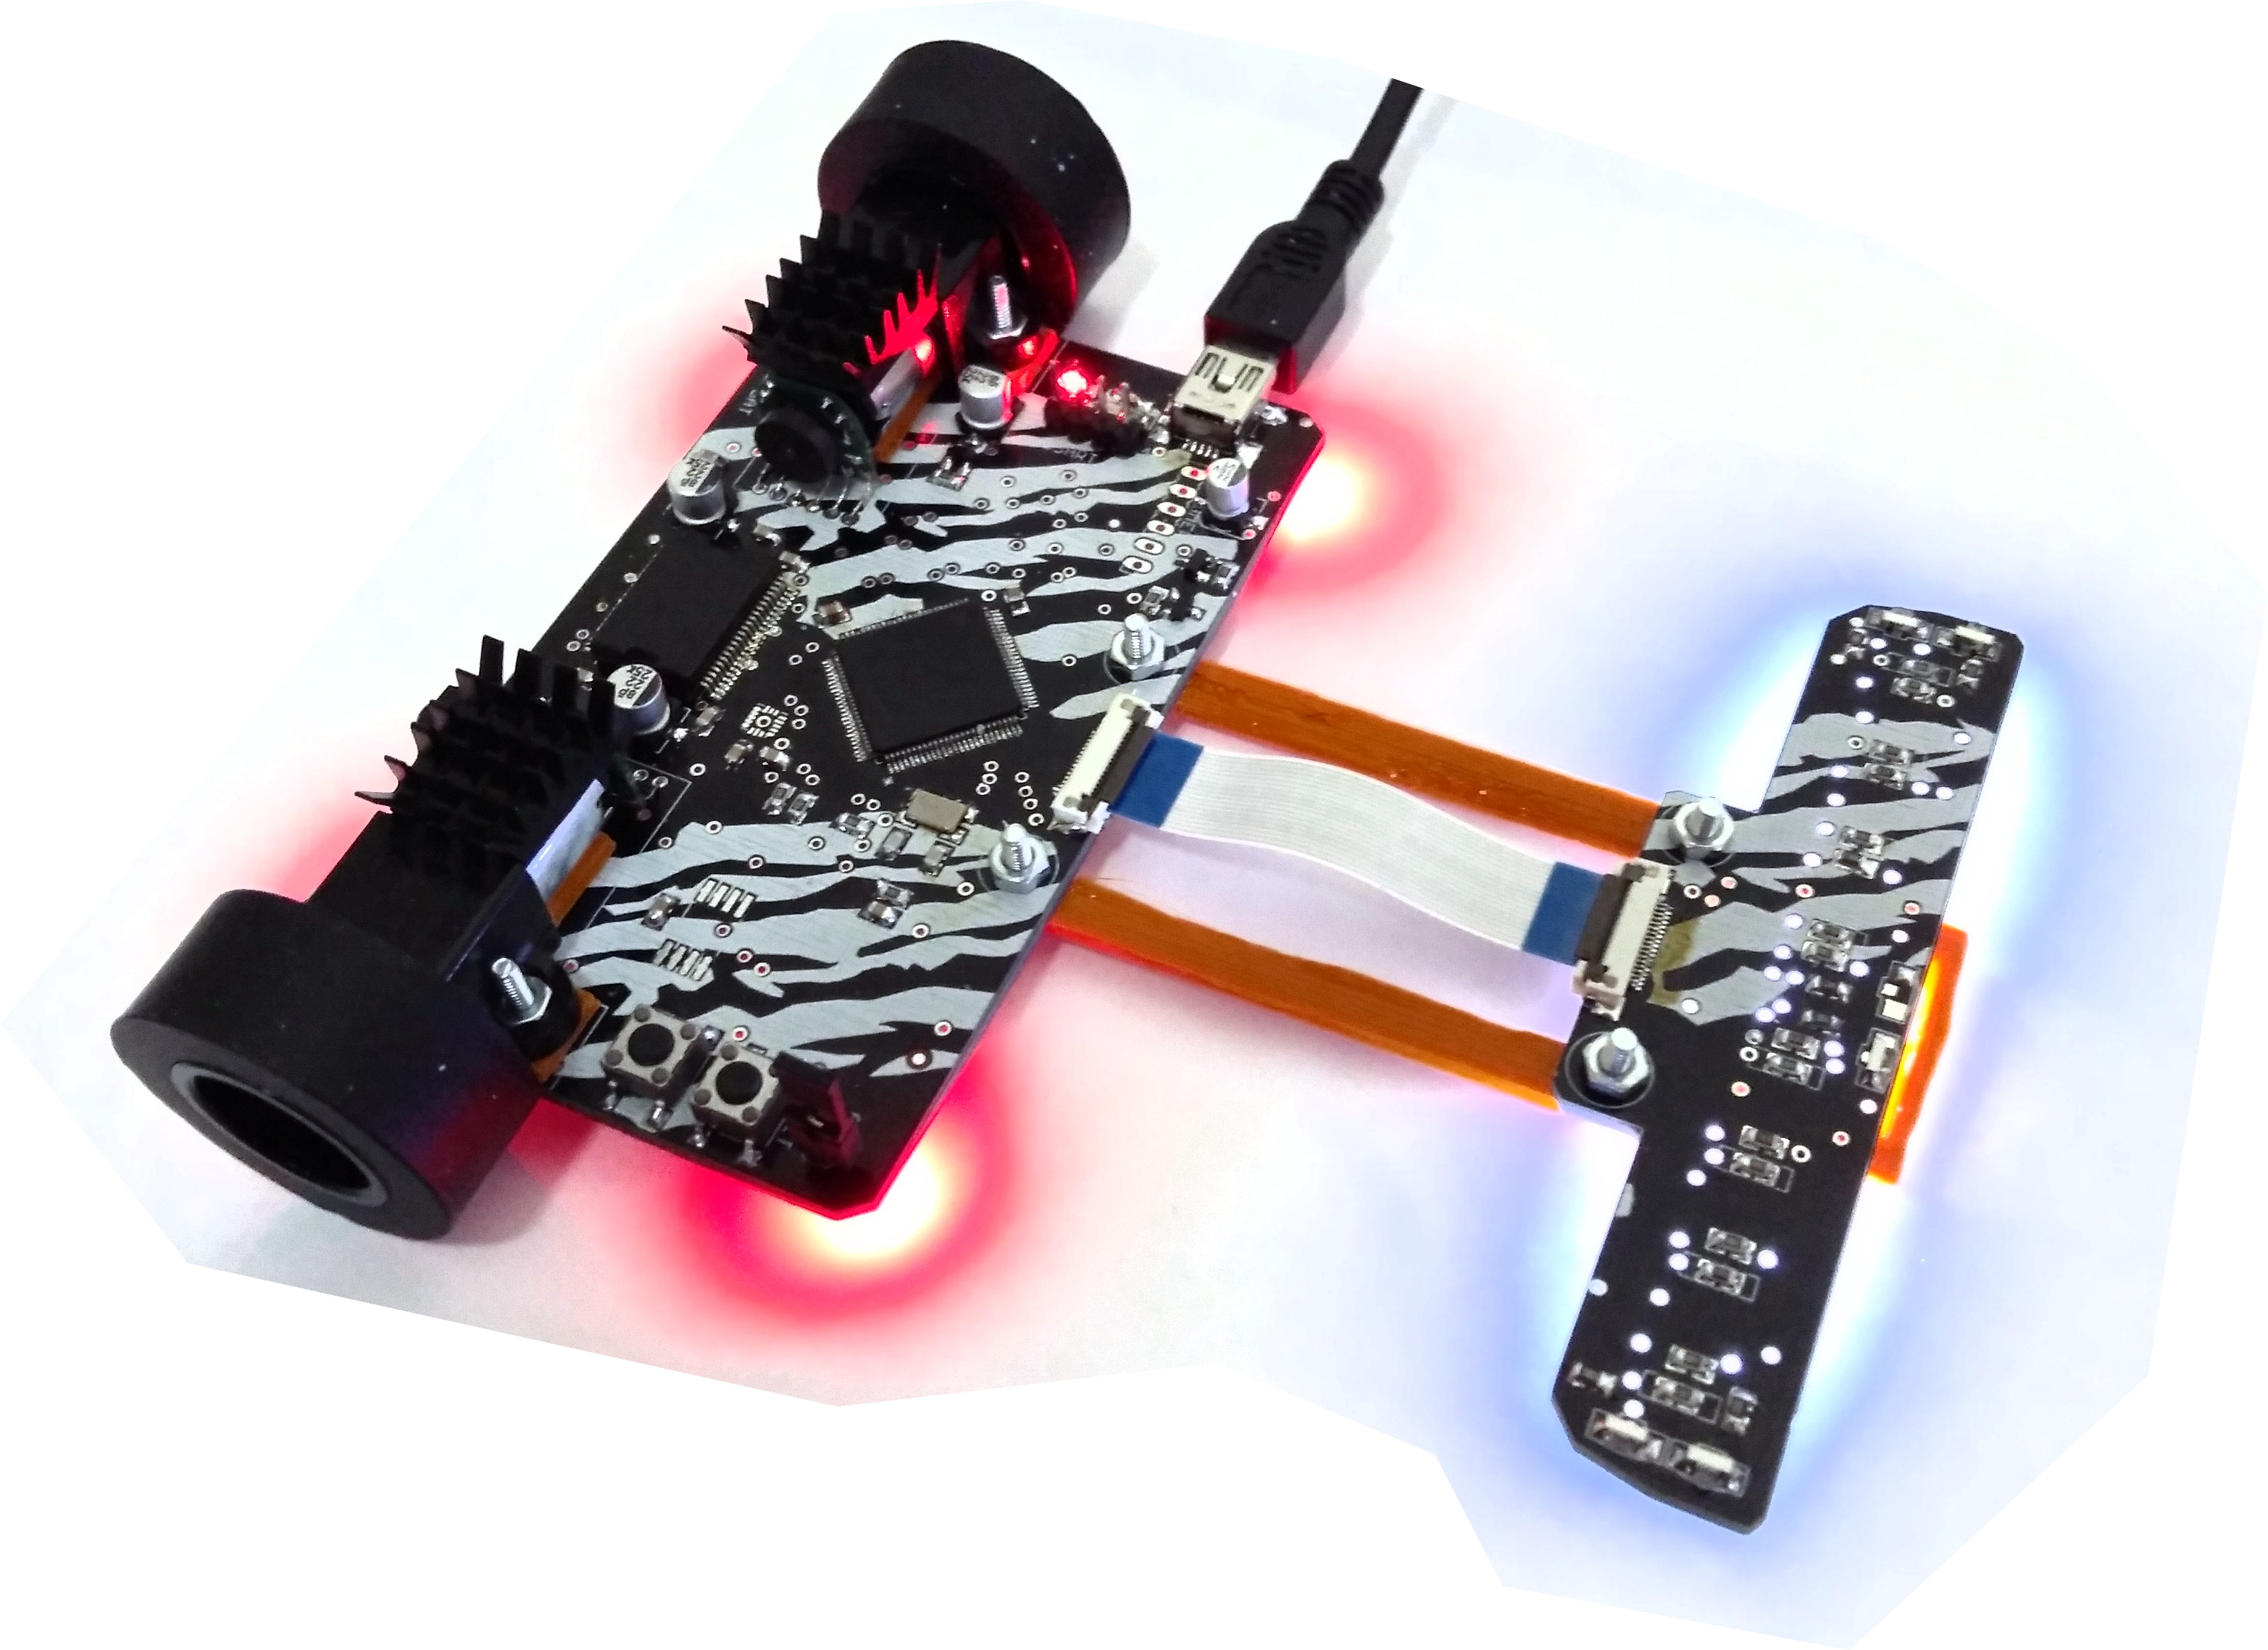
\includegraphics[scale=0.04]{../../pictures/robot_ascender.jpg}}
        ]{4cm}{3cm}{../../video/motko_uprising_neural_network_test.mp4}


    \end{column}

\end{columns}


\end{frame}



\begin{frame}{\bf Red blood cells trajectory prediction}

    Research group {\bf Cell in fluid} \\
    {\bf Mgr. Katarína Jasenčáková}, PhD thesis

    \begin{itemize}
      \item train DNN to predict RBC trajectory from past
      \item 15 conv layers network (6hours training on GTX1080ti)
      \item input : RBC position + 7 past frames + other cells position
      \item output: RBC predicted velocity
    \end{itemize}



    \begin{columns}
        \begin{column}{0.5\textwidth}

        \begin{figure}
          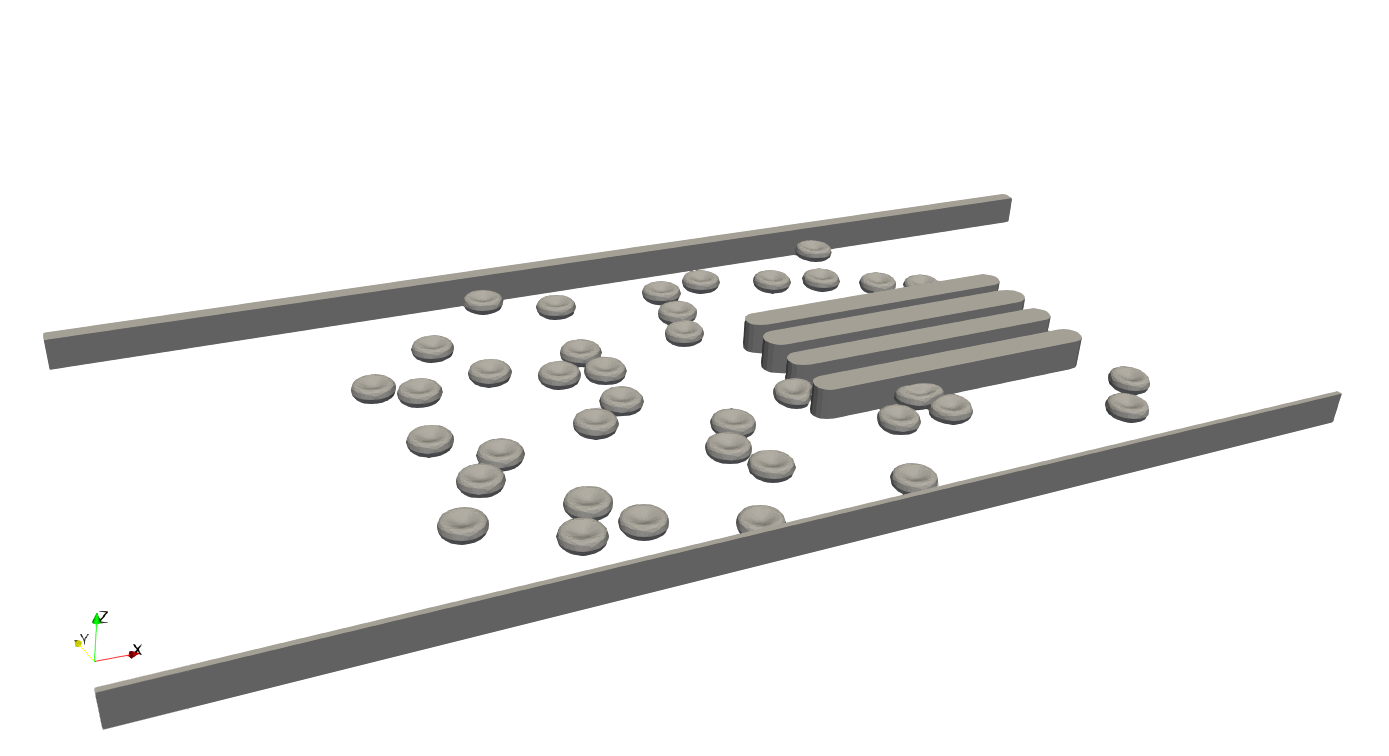
\includegraphics[scale=0.08]{../../pictures/rbc_channel.png}
        \end{figure}


        \end{column}

        \begin{column}{0.5\textwidth}  %%<--- here

            \includemovie[
              poster,
              autoplay,
              externalviewer,
              inline=false,
              text={ 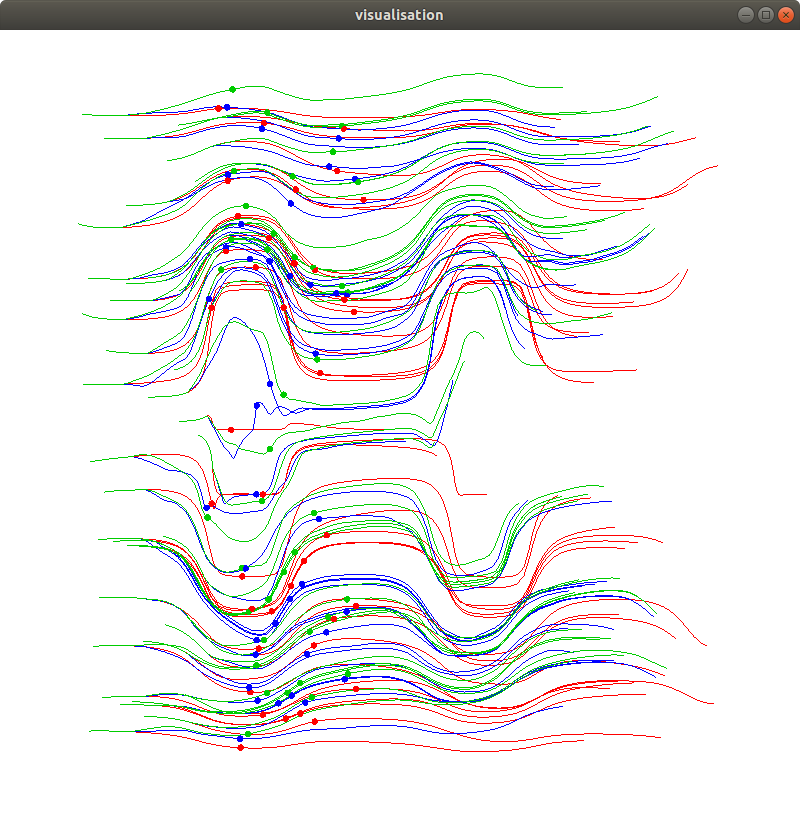
\includegraphics[scale=0.08]{../../diagrams/rbc_deep_network_6_7.png}}
            ]{2cm}{2cm}{../../video/cells_trajectory.mp4}


        \end{column}

    \end{columns}


    \begin{figure}
      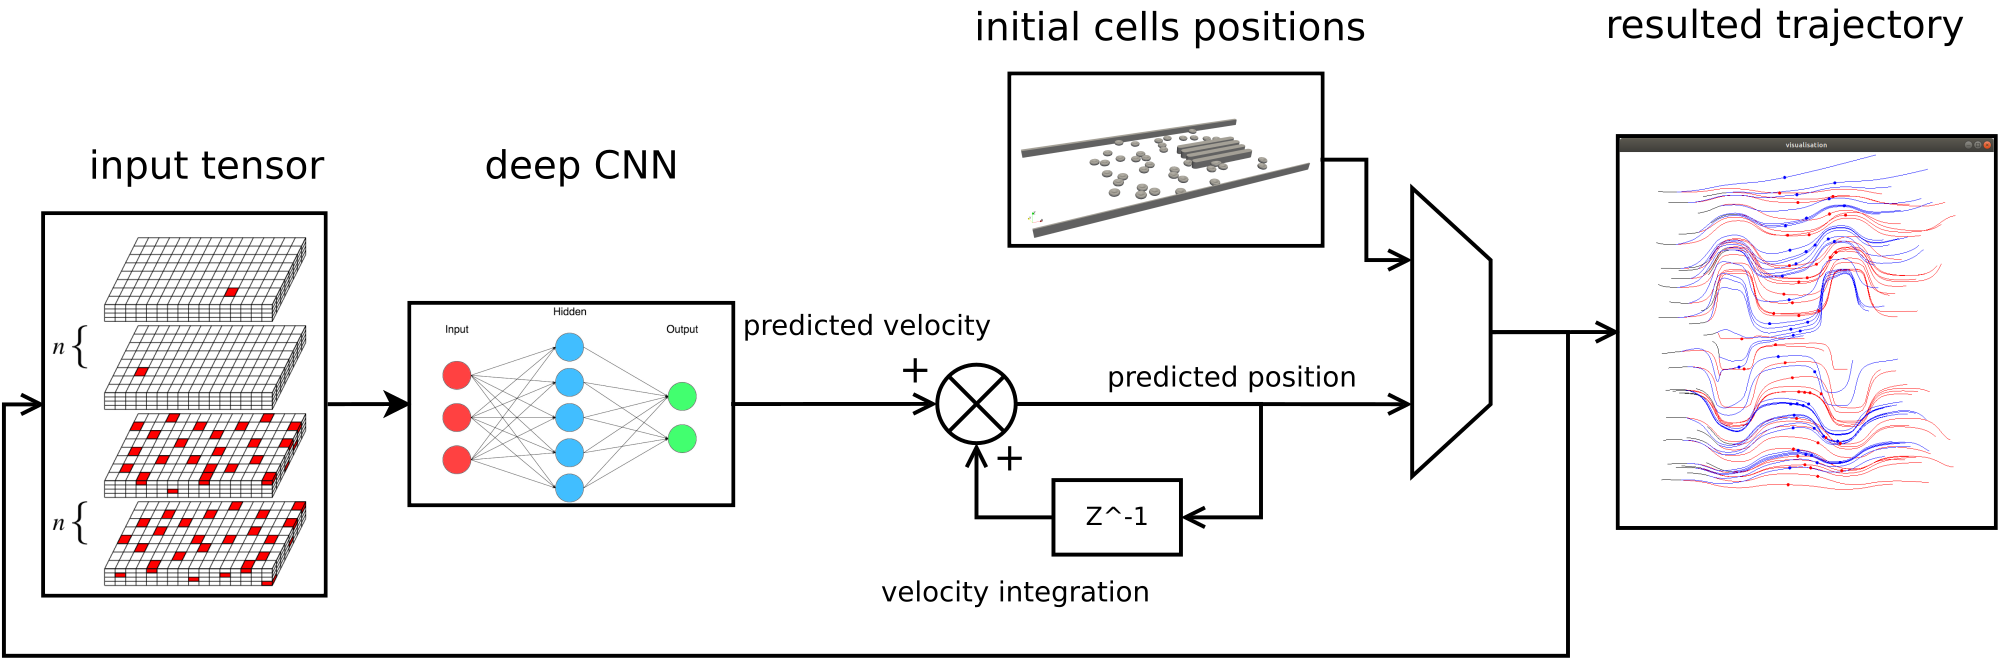
\includegraphics[scale=0.12]{../../diagrams/cells_prediction_velocity_integration.png}
    \end{figure}


\end{frame}


\begin{frame}{\bf Networks}


{\fontsize{5.2}{7}\selectfont

\begin{table}[]
\begin{tabular}{|l|l|l|l|l|l|l|l|l|}
\hline
\textbf{layer} & \textbf{net 0}                 & \textbf{net 1}                                                                 & \textbf{net 2}                                                                      & \textbf{net 3}                                                                      & \textbf{net 4}                                                                      & \textbf{net 5}                                                                      & \textbf{net 6}                                                                      & \textbf{net 7}                                                                      \\ \hline
0              & \cellcolor[HTML]{67FD9A}fc 256 & \cellcolor[HTML]{34CDF9}\begin{tabular}[c]{@{}l@{}}conv \\ 3x3x32\end{tabular} & \cellcolor[HTML]{FD6864}\begin{tabular}[c]{@{}l@{}}dense conv\\  3x3x8\end{tabular} & \cellcolor[HTML]{FD6864}\begin{tabular}[c]{@{}l@{}}dense conv\\  3x3x8\end{tabular} & \cellcolor[HTML]{FD6864}\begin{tabular}[c]{@{}l@{}}dense conv\\  3x3x8\end{tabular} & \cellcolor[HTML]{FD6864}\begin{tabular}[c]{@{}l@{}}dense conv\\  3x3x8\end{tabular} & \cellcolor[HTML]{FD6864}\begin{tabular}[c]{@{}l@{}}dense conv\\  3x3x8\end{tabular} & \cellcolor[HTML]{FD6864}\begin{tabular}[c]{@{}l@{}}dense conv\\  3x3x8\end{tabular} \\ \hline
1              & \cellcolor[HTML]{67FD9A}fc 64  & \cellcolor[HTML]{67FD9A}fc 64                                                  & \cellcolor[HTML]{FD6864}\begin{tabular}[c]{@{}l@{}}dense conv\\  3x3x8\end{tabular} & \cellcolor[HTML]{FD6864}\begin{tabular}[c]{@{}l@{}}dense conv\\  3x3x8\end{tabular} & \cellcolor[HTML]{FD6864}\begin{tabular}[c]{@{}l@{}}dense conv\\  3x3x8\end{tabular} & \cellcolor[HTML]{FD6864}\begin{tabular}[c]{@{}l@{}}dense conv\\  3x3x8\end{tabular} & \cellcolor[HTML]{FD6864}\begin{tabular}[c]{@{}l@{}}dense conv\\  3x3x8\end{tabular} & \cellcolor[HTML]{FD6864}\begin{tabular}[c]{@{}l@{}}dense conv\\  3x3x8\end{tabular} \\ \hline
2              & \cellcolor[HTML]{67FD9A}fc 32  & \cellcolor[HTML]{67FD9A}fc 32                                                  & \cellcolor[HTML]{FD6864}\begin{tabular}[c]{@{}l@{}}dense conv\\  3x3x8\end{tabular} & \cellcolor[HTML]{FD6864}\begin{tabular}[c]{@{}l@{}}dense conv\\  3x3x8\end{tabular} & \cellcolor[HTML]{FD6864}\begin{tabular}[c]{@{}l@{}}dense conv\\  3x3x8\end{tabular} & \cellcolor[HTML]{FD6864}\begin{tabular}[c]{@{}l@{}}dense conv\\  3x3x8\end{tabular} & \cellcolor[HTML]{FD6864}\begin{tabular}[c]{@{}l@{}}dense conv\\  3x3x8\end{tabular} & \cellcolor[HTML]{FD6864}\begin{tabular}[c]{@{}l@{}}dense conv\\  3x3x8\end{tabular} \\ \hline
3              & \cellcolor[HTML]{67FD9A}fc 3   & \cellcolor[HTML]{67FD9A}fc 3                                                   & \cellcolor[HTML]{FD6864}\begin{tabular}[c]{@{}l@{}}dense conv\\  3x3x8\end{tabular} & \cellcolor[HTML]{FD6864}\begin{tabular}[c]{@{}l@{}}dense conv\\  3x3x8\end{tabular} & \cellcolor[HTML]{FD6864}\begin{tabular}[c]{@{}l@{}}dense conv\\  3x3x8\end{tabular} & \cellcolor[HTML]{FD6864}\begin{tabular}[c]{@{}l@{}}dense conv\\  3x3x8\end{tabular} & \cellcolor[HTML]{FD6864}\begin{tabular}[c]{@{}l@{}}dense conv\\  3x3x8\end{tabular} & \cellcolor[HTML]{FD6864}\begin{tabular}[c]{@{}l@{}}dense conv\\  3x3x8\end{tabular} \\ \hline
4              &                                &                                                                                & \cellcolor[HTML]{34CDF9}conv 1x1x32                                                 & \cellcolor[HTML]{34CDF9}conv 1x1x16                                                 & \cellcolor[HTML]{34CDF9}conv 1x1x32                                                 & \cellcolor[HTML]{34CDF9}conv 1x1x16                                                 & \cellcolor[HTML]{34CDF9}conv 1x1x16                                                 & \cellcolor[HTML]{34CDF9}conv 1x1x32                                                 \\ \hline
5              &                                &                                                                                & \cellcolor[HTML]{67FD9A}fc 3                                                        & \cellcolor[HTML]{FD6864}\begin{tabular}[c]{@{}l@{}}dense conv\\  3x3x8\end{tabular} & \cellcolor[HTML]{67FD9A}fc 3                                                        & \cellcolor[HTML]{FD6864}\begin{tabular}[c]{@{}l@{}}dense conv\\  3x3x8\end{tabular} & \cellcolor[HTML]{FD6864}\begin{tabular}[c]{@{}l@{}}dense conv\\  3x3x8\end{tabular} & \cellcolor[HTML]{FD6864}\begin{tabular}[c]{@{}l@{}}dense conv\\  3x3x8\end{tabular} \\ \hline
6              &                                &                                                                                &                                                                                     & \cellcolor[HTML]{FD6864}\begin{tabular}[c]{@{}l@{}}dense conv\\  3x3x8\end{tabular} &                                                                                     & \cellcolor[HTML]{FD6864}\begin{tabular}[c]{@{}l@{}}dense conv\\  3x3x8\end{tabular} & \cellcolor[HTML]{FD6864}\begin{tabular}[c]{@{}l@{}}dense conv\\  3x3x8\end{tabular} & \cellcolor[HTML]{FD6864}\begin{tabular}[c]{@{}l@{}}dense conv\\  3x3x8\end{tabular} \\ \hline
7              &                                &                                                                                &                                                                                     & \cellcolor[HTML]{FD6864}\begin{tabular}[c]{@{}l@{}}dense conv\\  3x3x8\end{tabular} &                                                                                     & \cellcolor[HTML]{FD6864}\begin{tabular}[c]{@{}l@{}}dense conv\\  3x3x8\end{tabular} & \cellcolor[HTML]{FD6864}\begin{tabular}[c]{@{}l@{}}dense conv\\  3x3x8\end{tabular} & \cellcolor[HTML]{FD6864}\begin{tabular}[c]{@{}l@{}}dense conv\\  3x3x8\end{tabular} \\ \hline
8              &                                &                                                                                &                                                                                     & \cellcolor[HTML]{FD6864}\begin{tabular}[c]{@{}l@{}}dense conv\\  3x3x8\end{tabular} &                                                                                     & \cellcolor[HTML]{FD6864}\begin{tabular}[c]{@{}l@{}}dense conv\\  3x3x8\end{tabular} & \cellcolor[HTML]{FD6864}\begin{tabular}[c]{@{}l@{}}dense conv\\  3x3x8\end{tabular} & \cellcolor[HTML]{FD6864}\begin{tabular}[c]{@{}l@{}}dense conv\\  3x3x8\end{tabular} \\ \hline
9              &                                &                                                                                &                                                                                     & \cellcolor[HTML]{34CDF9}conv 1x1x32                                                 &                                                                                     & \cellcolor[HTML]{34CDF9}conv 1x1x32                                                 & \cellcolor[HTML]{34CDF9}conv 1x1x16                                                 & \cellcolor[HTML]{34CDF9}conv 1x1x32                                                 \\ \hline
10             &                                &                                                                                &                                                                                     & \cellcolor[HTML]{67FD9A}fc 3                                                        &                                                                                     & \cellcolor[HTML]{67FD9A}fc 3                                                        & \cellcolor[HTML]{FD6864}\begin{tabular}[c]{@{}l@{}}dense conv\\  3x3x8\end{tabular} & \cellcolor[HTML]{FD6864}\begin{tabular}[c]{@{}l@{}}dense conv\\  3x3x8\end{tabular} \\ \hline
11             &                                &                                                                                &                                                                                     &                                                                                     &                                                                                     &                                                                                     & \cellcolor[HTML]{FD6864}\begin{tabular}[c]{@{}l@{}}dense conv\\  3x3x8\end{tabular} & \cellcolor[HTML]{FD6864}\begin{tabular}[c]{@{}l@{}}dense conv\\  3x3x8\end{tabular} \\ \hline
12             &                                &                                                                                &                                                                                     &                                                                                     &                                                                                     &                                                                                     & \cellcolor[HTML]{FD6864}\begin{tabular}[c]{@{}l@{}}dense conv\\  3x3x8\end{tabular} & \cellcolor[HTML]{FD6864}\begin{tabular}[c]{@{}l@{}}dense conv\\  3x3x8\end{tabular} \\ \hline
13             &                                &                                                                                &                                                                                     &                                                                                     &                                                                                     &                                                                                     & \cellcolor[HTML]{FD6864}\begin{tabular}[c]{@{}l@{}}dense conv\\  3x3x8\end{tabular} & \cellcolor[HTML]{FD6864}\begin{tabular}[c]{@{}l@{}}dense conv\\  3x3x8\end{tabular} \\ \hline
14             &                                &                                                                                &                                                                                     &                                                                                     &                                                                                     &                                                                                     & \cellcolor[HTML]{34CDF9}conv 1x1x32                                                 & \cellcolor[HTML]{34CDF9}conv 1x1x64                                                 \\ \hline
15             &                                &                                                                                &                                                                                     &                                                                                     &                                                                                     &                                                                                     & \cellcolor[HTML]{67FD9A}fc 3                                                        & \cellcolor[HTML]{67FD9A}fc 3                                                        \\ \hline
\end{tabular}
\end{table}
}

\end{frame}


\begin{frame}{\bf Reinforcement learning}

\begin{columns}
\begin{column}{0.5\textwidth}

    \centering
    \includemovie[
      poster,
      autoplay,
      externalviewer,
      inline=false,
      text={ 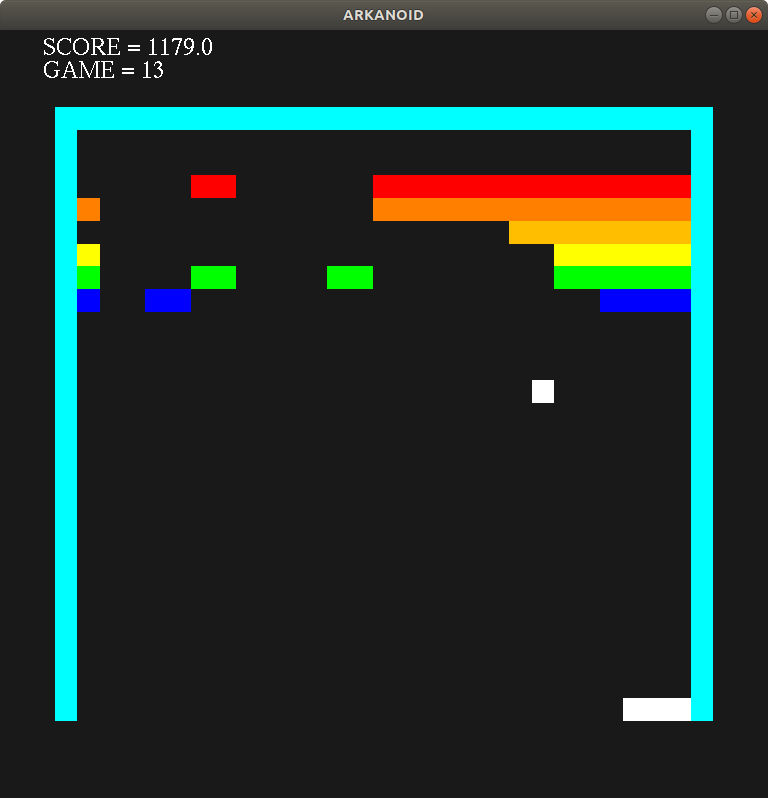
\includegraphics[scale=0.15]{../../diagrams/rl/arkanoid.png}}
    ]{4cm}{4cm}{../../video/rl_arkanoid.mp4}


  \begin{figure}[!htb]
    \centering
    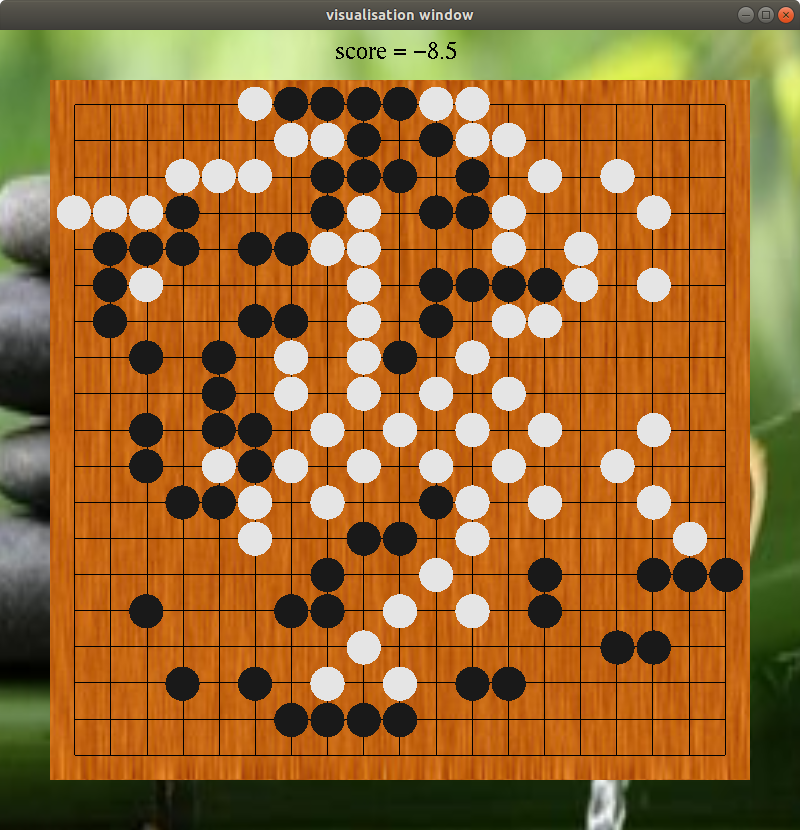
\includegraphics[scale=0.14]{../../diagrams/rl/go_board.png}
  \end{figure}


\end{column}
\begin{column}{0.5\textwidth}  %%<--- here

      \begin{itemize}
      \item {\bf playing Atari}
      \item {\bf playing Doom} -> scheduled on next month
      \item {\bf playing GO}
                              {
                                  \scriptsize
                                  {
                                    \begin{itemize}
                                      \item {\bf supervised training} - train game using Masters games
                                      \item {\bf reinforcement learning} - let play two networks against each other
                                    \end{itemize}
                                  }
                               }
    \end{itemize}


    \begin{figure}[!htb]
      \centering
      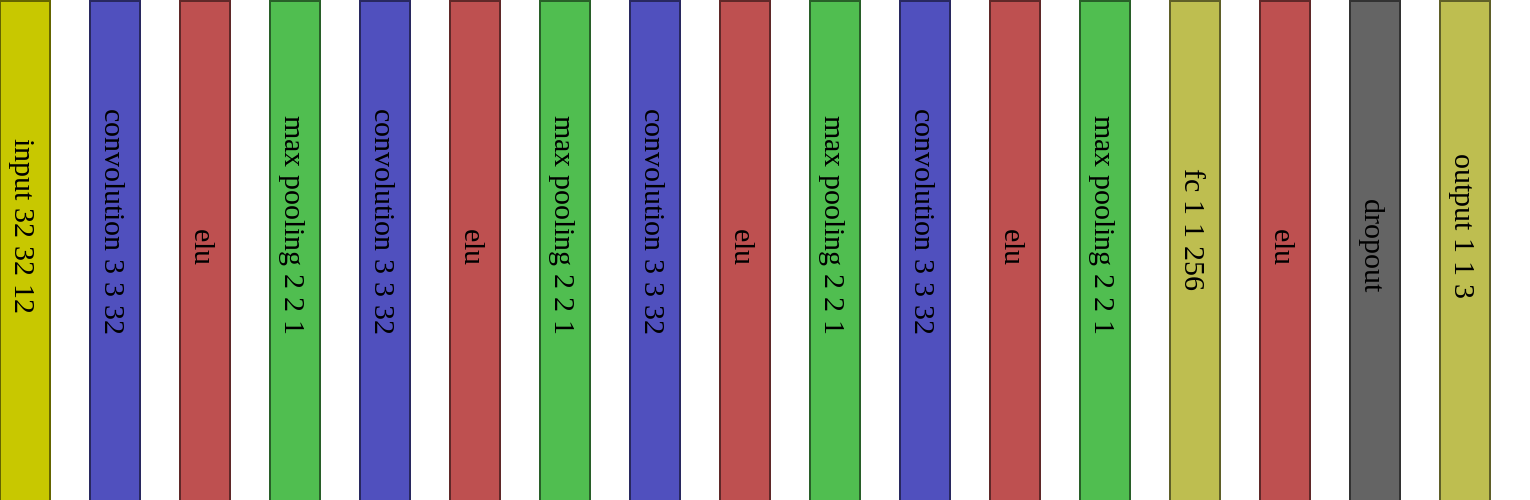
\includegraphics[scale=0.12]{../../diagrams/rl/net_1.png}
    \end{figure}

\end{column}
\end{columns}

\end{frame}



\begin{frame}{\bf GO Network architecture}
we need to go much deeper for GO
\begin{itemize}
  \item {\bf 28, 35 layers} \\ dense blocks + feature pooling layer
  \item {\bf input} \\ 4 matrices $19x19$: black stones, white stones, empty fields, active player
  \item {\bf output} \\ recommended moves 19x19 + 1 for pass = 362 outputs

\end{itemize}

  \begin{figure}[!htb]
    \centering
    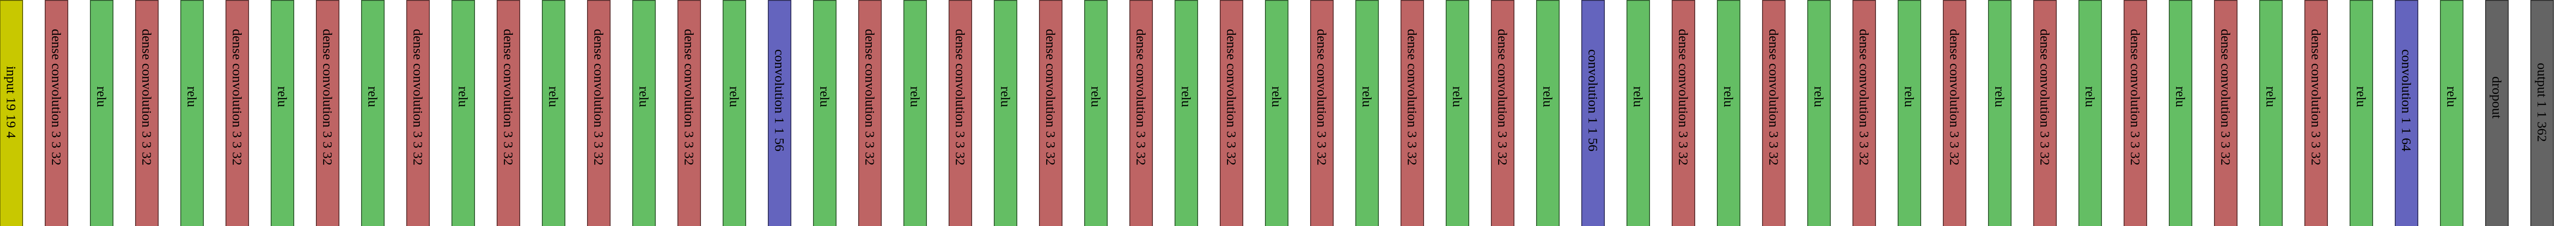
\includegraphics[scale=0.06]{../../diagrams/net_go_1_28_layers.png}
  \end{figure}

  \begin{figure}[!htb]
    \centering
    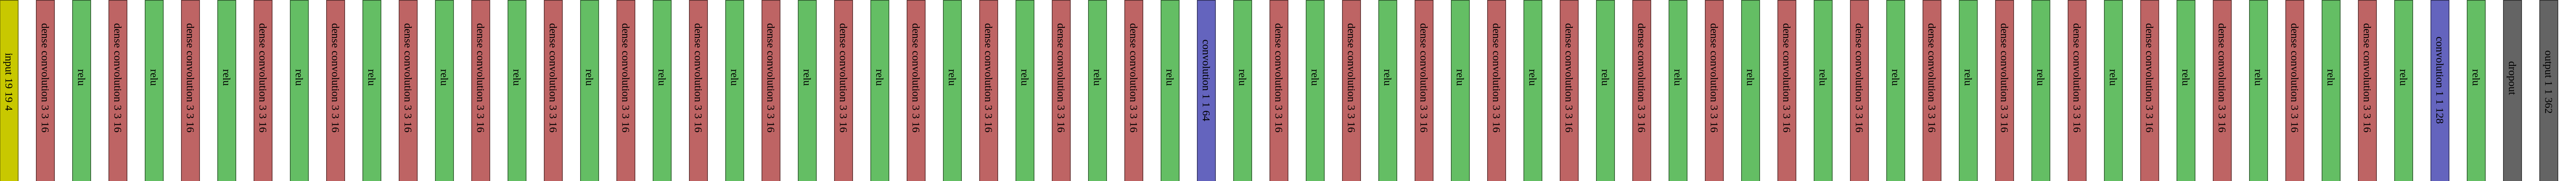
\includegraphics[scale=0.06]{../../diagrams/net_go_5_35_layers.png}
  \end{figure}

\end{frame}




\begin{frame}{\bf Other stuff}

\begin{columns}
\begin{column}{0.5\textwidth}

\begin{figure}[!htb]
  \centering
  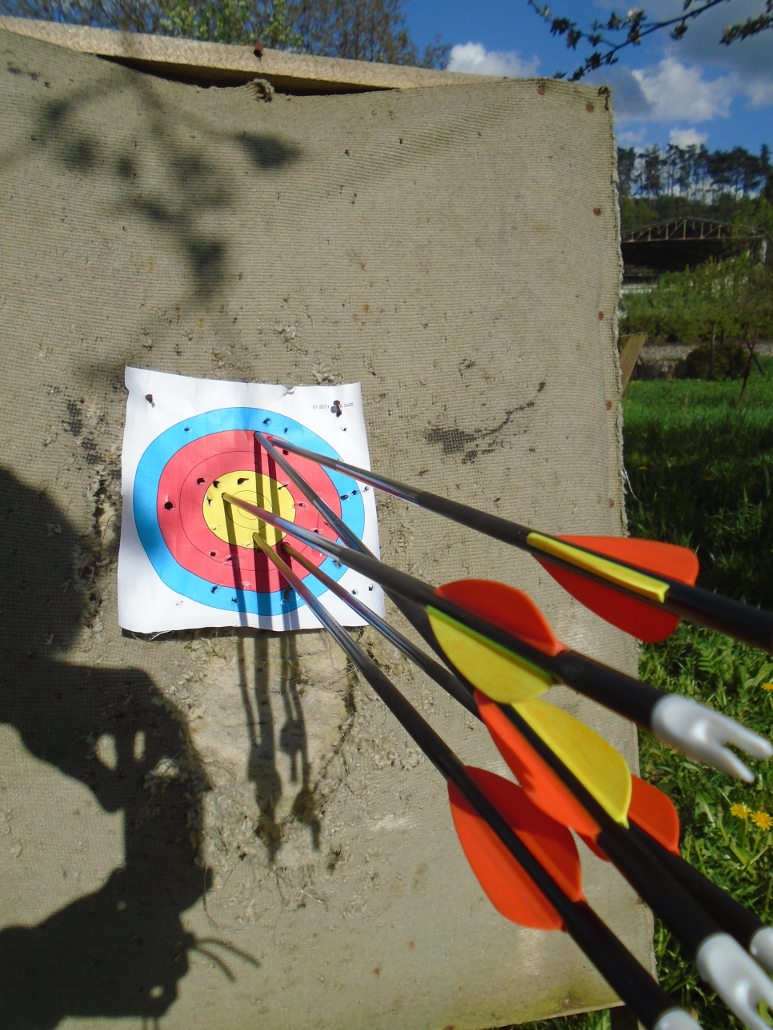
\includegraphics[scale=0.4]{../../pictures/me_03.jpg}
\end{figure}

\begin{figure}[!htb]
  \centering
  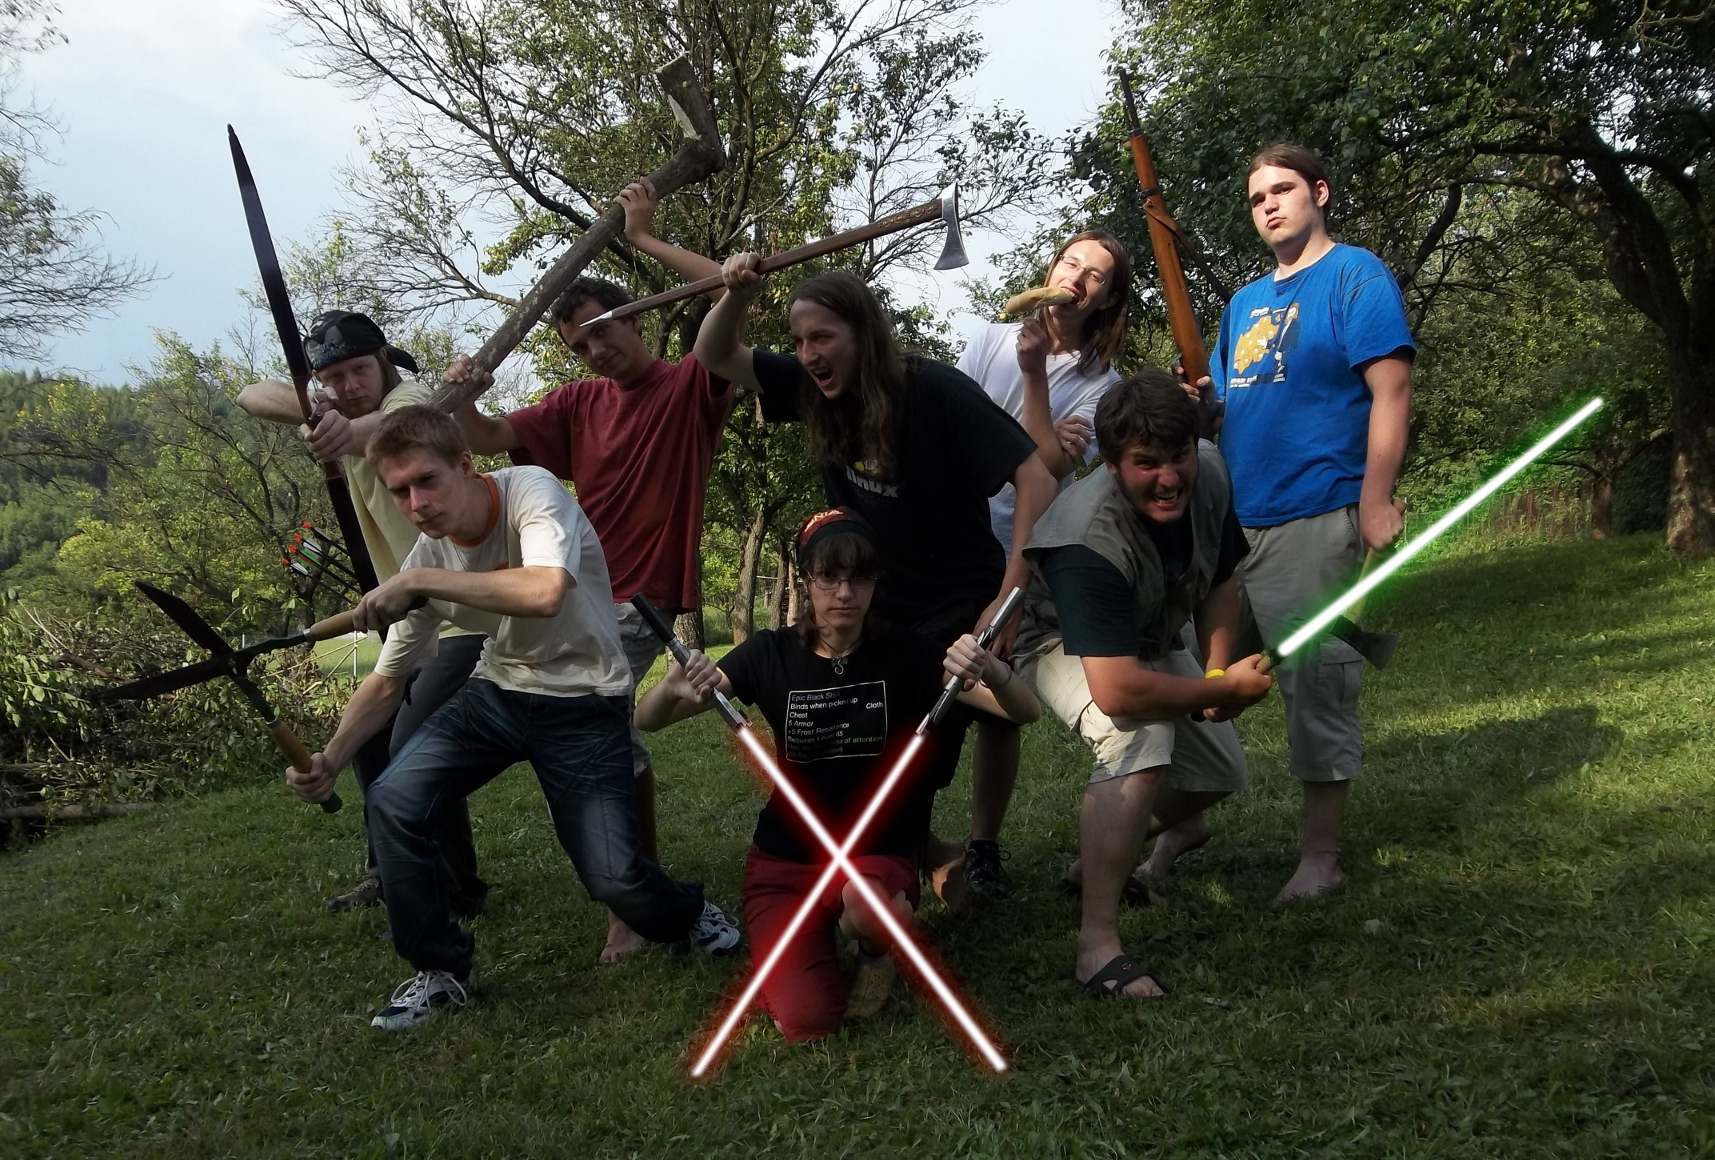
\includegraphics[scale=0.1]{../../pictures/me_04.jpg}
\end{figure}

\end{column}
\begin{column}{0.5\textwidth}  %%<--- here

\begin{itemize}
  \item hiking, running
  \item archery, aikido
  \item caving, climbing
\end{itemize}

    \begin{figure}[!htb]
      \centering
      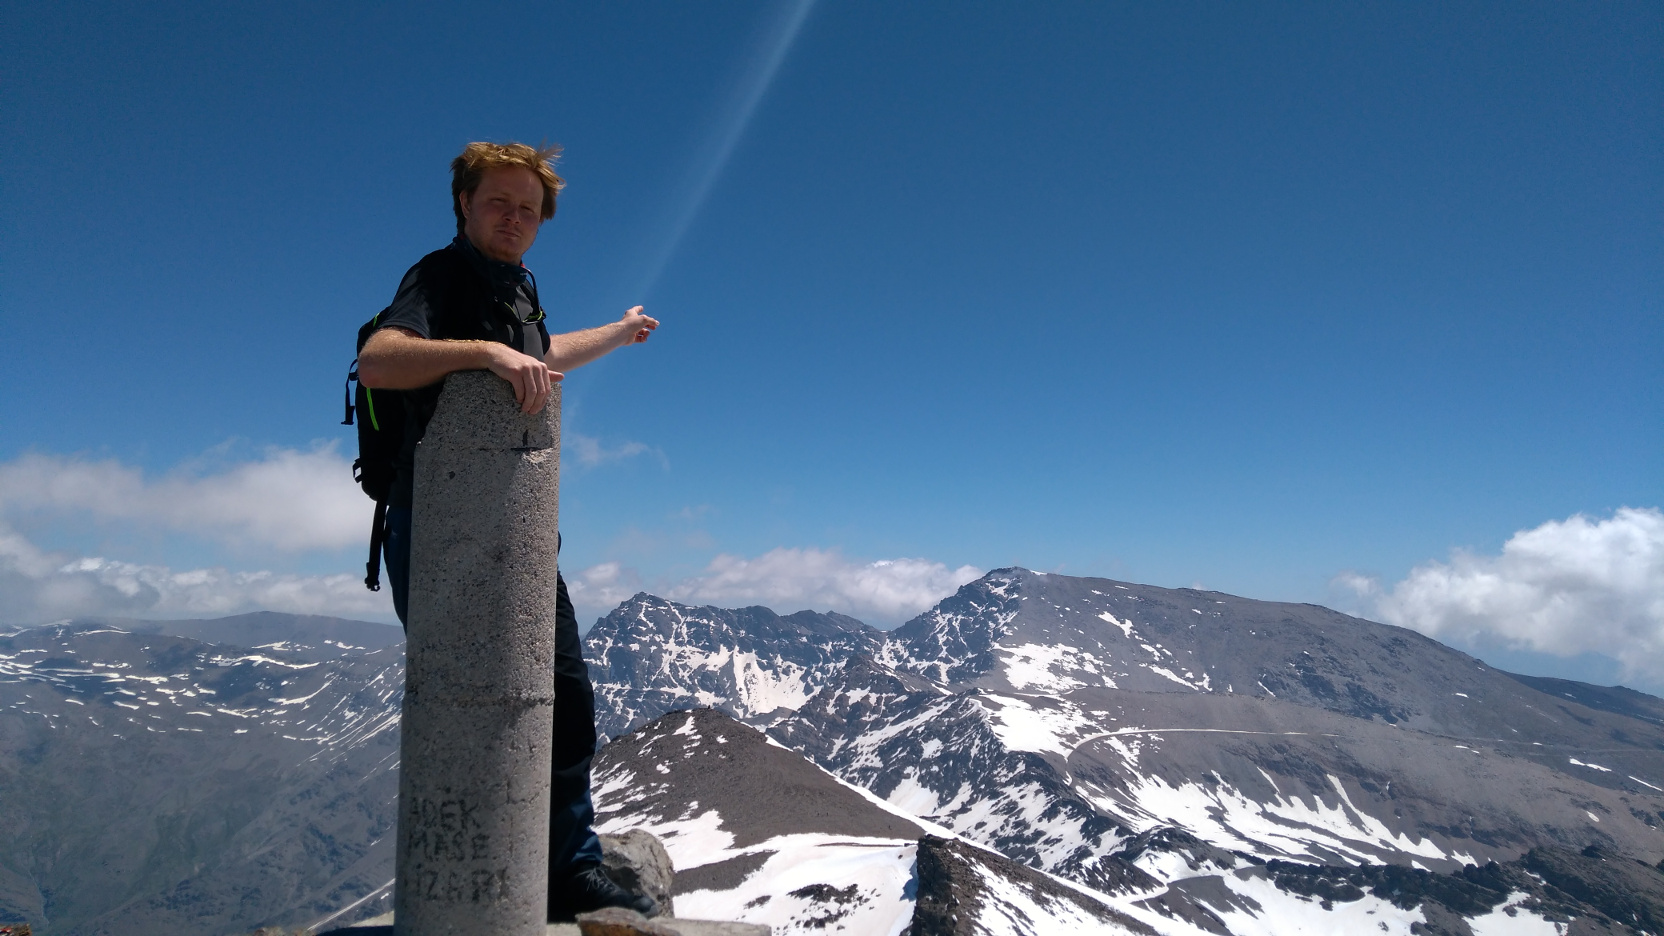
\includegraphics[scale=0.08]{../../pictures/me_01.jpg}
    \end{figure}
    \begin{figure}[!htb]
      \centering
      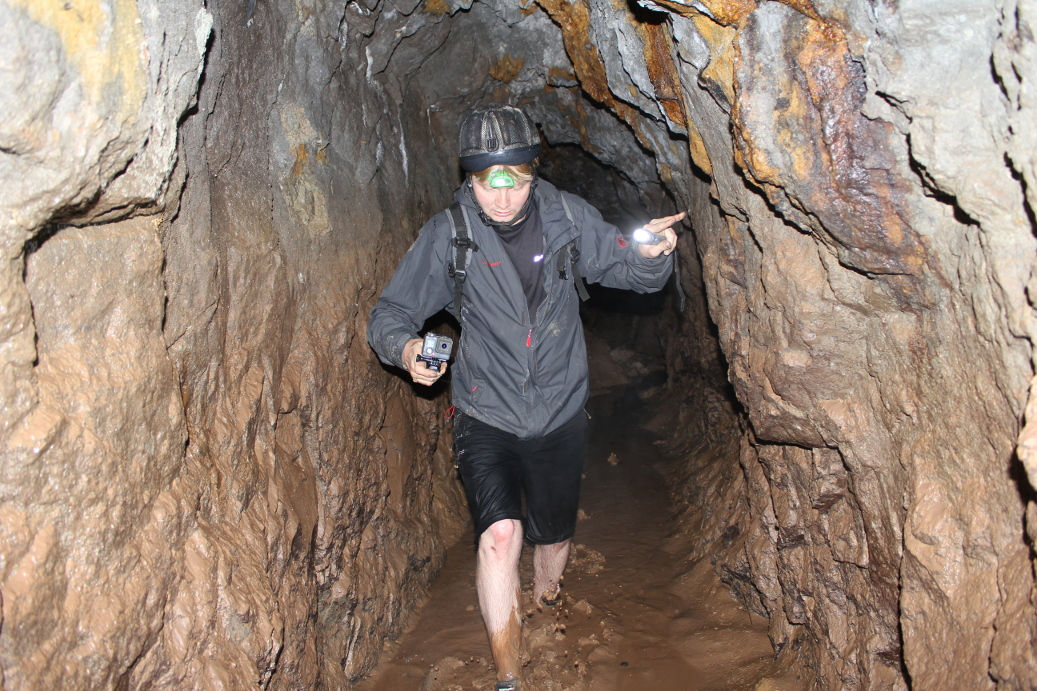
\includegraphics[scale=0.1]{../../pictures/me_02.jpg}
    \end{figure}


\end{column}
\end{columns}


\end{frame}




\end{document}
